\documentclass{article}
\usepackage[utf8]{inputenc}
\usepackage{graphicx}

\author{Bijan Varjavand}
\title{LabNotebook}
\date{February 7, 2017}

\begin{document}

\maketitle

\section{Objectives}

The goal this lab was to recognize the relationships between temperature and conductivity for different types of metals.

\section{Setup}

Samples were provided by the lab, which were an assortment of many different types of rod. Same as in Lab 1A.
\subsection{Materials}

Brass, Phosphor Bronze, and Aluminum were the three materials our group chose.
\subsection{Tools}

Our group used power sources and multimeters for our measurements, as well as a thermocouple and a furnace.
\section{Procedure}

We added a thermocouple, wrapping it around the sample. This was to measure voltage, which we can convert to
temperature. The integrated labview software is able to generate the necessary data, and automatically
does all the conversions we need. A diagram of this setup is shown below

\begin{figure}[h!]
\centering
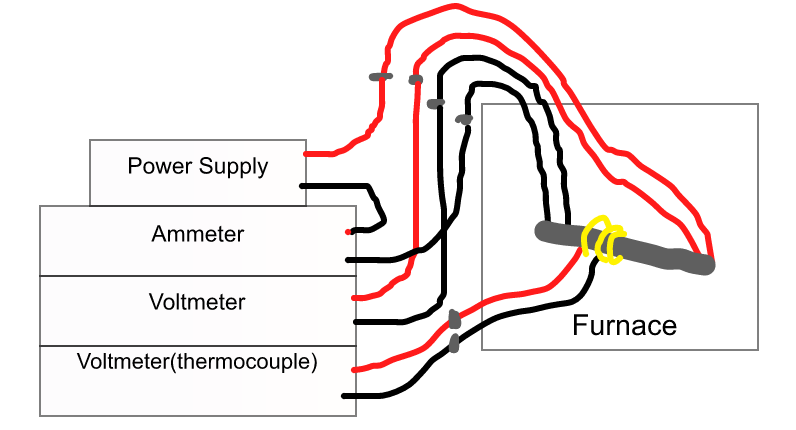
\includegraphics[scale=0.5]{circuit2.png}
\end{figure}

\section{Results}

The data collected made it possible to plot temperature vs conductivity, shown below.

\begin{figure}[h!]
\centering
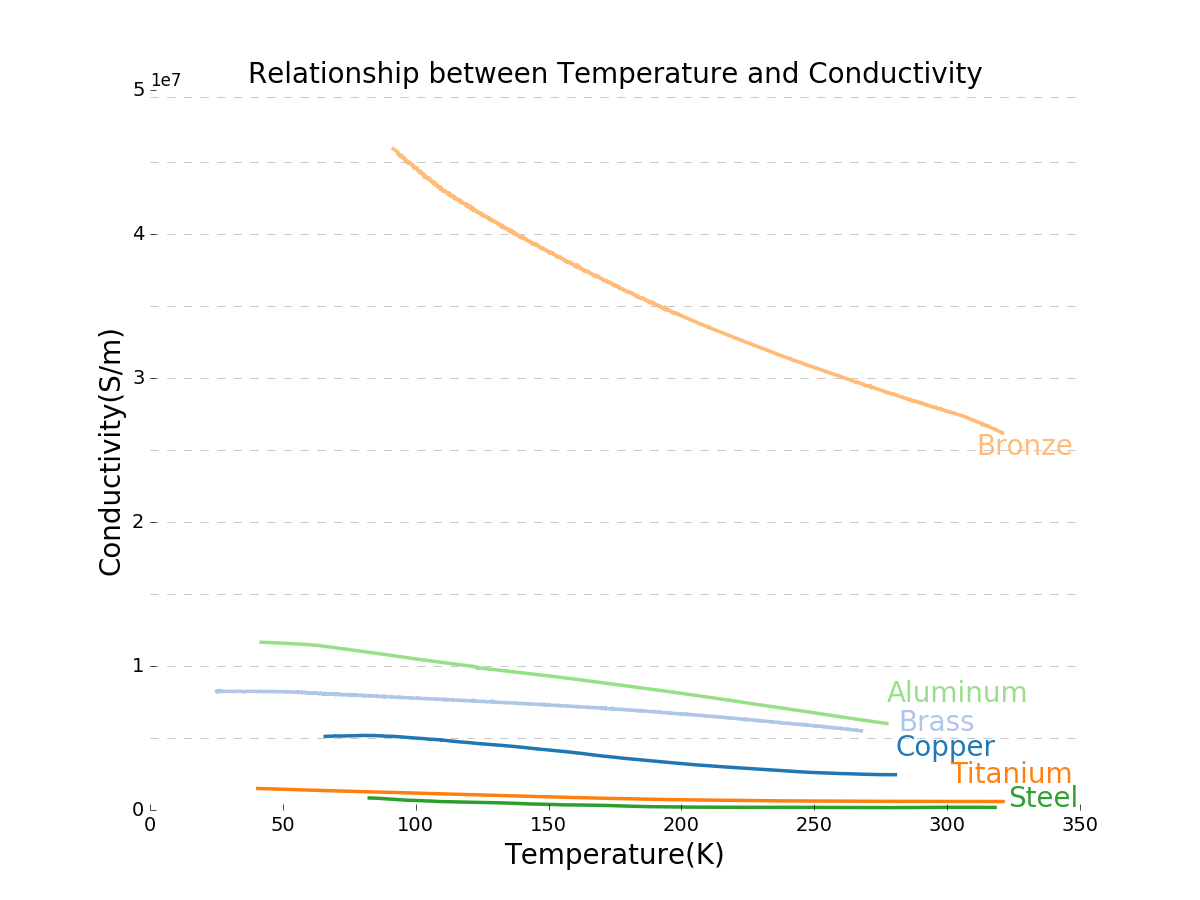
\includegraphics[scale=0.4]{lab1b.png}
\end{figure}

\section{Observations}

The general relationship we expect, which was the inverse relationship between temperature and conductivity, is seen to hold. We can also see how this varies between different types of materials.
\end{document}